% sample.tex
\documentclass[20pt]{beamer}
\usetheme{default}
\beamertemplatenavigationsymbolsempty
\usepackage{listings}

\definecolor{darkgreen}{rgb}{0,.5,0}

\lstset{language=Lisp,
  basicstyle=\ttfamily\scriptsize,
  stringstyle=\color{red},
  commentstyle=\color{darkgreen},
  breaklines = true,
}

\title[]{Lisp}
\author[Jon]{https://github.com/
JonChesterfield/lisp-meetup.git}

\begin{document}

\begin{frame}
  \titlepage
\end{frame}

\begin{frame}{Lisp is mathematics}
  \begin{itemize}
  \item John McCarthy, MIT, April 1960
  \item Instantiation of the $\lambda$ calculus
  \item A basis set for computation
  \end{itemize}
\end{frame}

\begin{frame}{Lisp is a language}
  \begin{itemize}
  \item (car cdr cons if quote eq atom)
  \item Kernel
  \item Scheme
  \item Emacs lisp
  \item Common lisp
  \item Clojure
  \end{itemize}
\end{frame}

\begin{frame}{Lisp is whatever you want}
  \begin{itemize}
  \item Dynamically \& statically typed
  \item Compiled \& interpreted
  \item Deterministic \& unpredictable
  \item Uniform \& disambiguated
  \item Flexible \& performant
  \item Customizable \& standardised
  \end{itemize}
\end{frame}

\begin{frame}{Lisp can be what I want}
  \begin{itemize}
  \item Referentially transparent
  \item Implicitly multithreaded
  \item Implicitly distributed
  \item Faster than C++
  \item Clearer than Python
  \item Provably correct
  \end{itemize}
\end{frame}

\begin{frame}{Lisp is a compiler's IR}
  \begin{figure}
    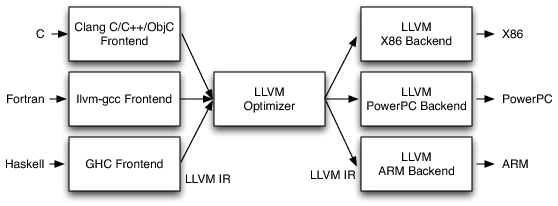
\includegraphics[height=4.2cm]{LLVMCompiler1.png}
    \caption{I can't work out who to cite!}
  \end{figure}
\end{frame}

\begin{frame}[fragile]{So it tends to look like}
  \begin{lstlisting}
(define (fact n)
  (if (<= n 1)
    1
    (* n (fact (- n 1)))))
(defun fact (n)
  (if (<= n 1)
    1
    (* n (fact (- n 1)))))
(defn fact [x]
  (loop [n x f 1]
    (if (<= n 1)
      f
      (recur (dec n) (* f n)))))
  \end{lstlisting}
\end{frame}

\begin{frame}{And that's not so bad}
  \begin{itemize}
  \item sum (a, b, c) $\approx$ (sum a b c)
  \item (a + b + c + d) $\approx$ (+ a b c d)
  \item func two (x) \{ return 2 * x; \} $\approx$ (define two (x) (* 2 x))
  \item (8 == two(4)) $\approx$ (= 8 (two 4))
  \item Maybe an hour to adjust.
  \end{itemize}
\end{frame}

\begin{frame}{Where to start?}
  \begin{itemize}
  \item Scheme $=>$ guile, racket, chicken, gambit
  \item Common lisp $=>$ sbcl, ccl, gcl
  \item Clojure $=>$ Clojure
  \item Elisp $=>$ Emacs
  \item Kernel $=>$ Write your own
  \end{itemize}
\end{frame}

\begin{frame}{Most likely to be...}
  \begin{itemize}
  \item Dynamically typed
  \item Lexically scoped
  \item Garbage collected
  \item Adequately fast
  \item Syntactically customisable
  \item Semantically customisable
  \end{itemize}
\end{frame}

\begin{frame}[fragile]{Dynamically typed}
  \begin{lstlisting}
(define (dyn val)
  (if (number? val)
    42
    ``life''))
(dyn 5)   ; => 42
(dyn dyn) ; => ``life''

(define var 42)
var       ; => 42
(set! var (lambda () (``life'')))
var       ; => #<procedure var ()>
(var)     ; => ``life''
  \end{lstlisting}
\end{frame}

\begin{frame}[fragile]{Lexically scoped}
  \begin{lstlisting}
    (define (print x)
      (begin (write x) (newline)))
    (define (what x)
      (if (= a 1)
        (print ``Lexical'')
        (print ``Dynamic'')))
    (let ((a 1))
      (let ((f (lambda () (what a))))
        (let ((a 2))
          (f)))) ; ``Lexical''
  \end{lstlisting}
\end{frame}

\begin{frame}{Garbage collected}
  \begin{itemize}
  \item Objects appear to live forever
  \item Unwind-protect $\approx$ (with $|$ using)
  \item Unwind-protect $\neq$ (with $|$ using)
  \end{itemize}
\end{frame}

\begin{frame}{Syntactically customisable}
  \begin{itemize}
  \item Clojure [1 2] \& $\{:a\ 1, :b\ 2\}$
  \item Racket \#(1 2) \& $(hash\ 'a\ 1\ 'b\ 2)$
  \item Common lisp has reader macros
  \item Scheme has srfi-10 e.g. $\#,(foo)$
  \item I'd rather use a DSL \& parser
  \end{itemize}
\end{frame}

\begin{frame}{Semantically customisable}
  \begin{itemize}
  \item call-with-current-continuation
  \item defmacro
  \item syntax-rules
  \item fexpr
  \item hack up the compiler
  \end{itemize}
\end{frame}

\begin{frame}[fragile]{Example 0}
  \begin{lstlisting}
(define (fib n)
  (cond ((= n 0) 0)
        ((= n 1) 1)
        (#t (+ (fib (- n 1))
               (fib (- n 2))))))
(map fib '(0 1 2 3 4 5 6  7  8))
     ; => (0 1 1 2 3 5 8 13 21)
  \end{lstlisting}
\end{frame}

\begin{frame}[fragile]{Example 1}
  \begin{lstlisting}
(define eval-print
  (lambda (X)
    (begin
      (display X)
      (display ``=>'')
      (display (primitive-eval X))
      (newline))))
(eval-print '(letrec ((fact (lambda (n)
  (if (<= n 1) 1 (* n (fact (- n 1)))))))
    (fact 6))) ; (letrec...) => 720
  \end{lstlisting}
\end{frame}

\begin{frame}[fragile]{Example 2}
  \begin{lstlisting}
(define list-iter  (lambda (lst)
  (define iter (lambda () (call/cc cs)))
    (define cs
      (lambda (ret)
        (for-each (lambda (element)
          (set! ret (call/cc (lambda
            (resume-here)
              (set! cs resume-here)
              (ret element)))))
          lst)
        (ret 'EOL)))
    iter))
(define it (list-iter '(1 ``foo'' 3)))
(it) ; => 1
(it) ; => ``foo''
  \end{lstlisting}
\end{frame}

\begin{frame}{Cheat sheet}
  \begin{itemize}
  \item (quote 1 2 3) $==$ '(1 2 3)
  \item (list 1 2 3 ) $==$ '(1 2 3)
  \item (define f (lambda (x) (* 2 x)))
  \item (if (equal? 1 2) 19 42)
  \item (car (cons 1 2 3)) $=>$ 1
  \item (cdr (cons 1 2 3)) $=>$ (2 3)
  \item (display ``foobar'')
  \end{itemize}
\end{frame}

\end{document}
